\chapter{Data Decomposition}
\label{chap:data-decomp}

\section{Background}

It has been mentioned several times already in this thesis, but it bears
reminding the reader once again --- one of the imminent challenges for Monte
Carlo, as well as deterministic, methods is coping with limited amounts of
memory. While the availability of great amounts of processing power might
otherwise enable us to perform simulations with remarkable fidelity, the memory
requirements for such simulations will often exceed that available. For a
high-fidelity realistic LWR simulation, tally data alone will likely require
terabytes of memory (see discussion in \autoref{sec:tally-memory}). This problem
is exacerbated by the fact that current parallel methods still generally rely on
each program instance storing the full geometry, interaction cross sections, and
tally data in memory.

There is of course good reason to use full memory replication --- each process
can simulate particles independently\footnote{This is strictly only true in a
  fixed source calculation. In an eigenvalue calculation, there is a dependency
  between fission source iterations.} of one another and the tally results can
be collected at the end of the simulations. However, it is clear that some
method for avoiding replication of cross section and tally data must be an
essential component in any strategy to simulate reactor models with Monte
Carlo. Two algorithms have been proposed in the literature that do offer the
potential to avoid replication and furthermore decompose tally data across many
processors: domain decomposition and data decomposition.

In \autoref{chap:domain-decomp}, we presented a theoretical analysis of domain
decomposed Monte Carlo particle transport simulations looking at the effect of
load imbalances on the total simulation time. The analysis demonstrated that
load imbalances in domain decomposed simulations arise from two different
phenomena: non-uniform particle densities and non-uniform spatial leakage. It's
important to draw attention to the fact that even if we assumed zero latency and
zero inverse bandwidth (i.e. an infinitely fast network), the load imbalance
penalty does not disappear --- it is a physical artifact. In this chapter, we
now draw our attention to an algorithm which avoids load balancing issues by
keeping individual particles local to a single process while explicitly
decomposing the tally data.

\subsection{Data decomposition}

While a considerable amount of work and analysis has been carried out on domain
decomposition, very little work has focused on data decomposition to-date. The
basic concept of data decomposition is that a disjoint subset of the processes
in a simulation act as \emph{servers}, sending and/or receiving data to
\emph{compute processes} as needed\footnote{It is not absolutely necessary to
  have the servers and compute processes be mutually exclusive, but for the sake
  of simplicity we will consider them to be disjoint in the current work.}. In
its most general form, the data could be geometry, cross sections, and/or
tallies. The compute processes handle the actual transport of particles from
birth to death and communicate with the servers as needed. Thus, we see that
data decomposition does have some similarities to domain decomposition in the
sense that the compute processes are still tracking particles independently of
one another. However, particles are never transferred from one process to
another.

The potential for data decomposition to alleviate per-node memory restrictions
had been identified by Brown and Martin as early as 2004
\cite{trans-brown-2004}, but to-date it appears not to have been demonstrated or
even analyzed. Some early scoping work was done to investigate whether remote
memory access would be suitable for data decomposition algorithms
\cite{pnst-romano-2011}. However, these preliminary works focused more on
decomposing geometry and cross section data. In this paper, we take a first look
at an algorithm designed not to decompose geometry or cross section data but
rather to decompose large tally data.

We note that the data decomposition method can generally be considered to be a
partitioned global address space (PGAS) programming model. While PGAS models
have been discussed widely within the computer science community, there have not
yet been many practical applications using PGAS techniques or languages. A paper
being presented at the IEEE International Conference on High Performance
Computing, however, looks at the use of a partitioned global address space model
for quantum Monte Carlo simulations \cite{hipc-niu-2012}.

The analysis and results in this chapter are included in a paper submitted for
publication in \emph{Journal of Computational Physics} \cite{jcp-romano-2013}.

%%%%%%%%%%%%%%%%%%%%%%%%%%%%%%%%%%%%%%%%%%%%%%%%%%%%%%%%%%%%%%%%%%%%%%%%%%%%%%%%
\subsection{Tally Server Algorithm}
\label{sec:tally-server-algorithm}

During a Monte Carlo simulation, estimates of physical parameters are made by
keeping running sums of scores from events such as collisions or particle
tracks. These running sums are referred to as \emph{tallies}. The theory and
implementation of tallies was discussed at length in \autoref{sec:tallies}. The
simplicity of tally incrementing makes it amenable to an atomic fetch-and-add
operation (whether this be a CPU instruction or a remote direct memory access
operation). Normally, tallies are stored in local memory. Synchronization
between processors is typically performed only after simulating a predetermined
number of particles, referred to as a \emph{batch}. However, since tally data is
not needed for determining the random walk of a particle, it can be stored
remotely. For the sake of simplicity, we will look at an algorithm where the
tally data is stored in the address space of a process whose sole purpose is to
receive scores from other processes and increment the tallies accordingly. These
processes are called \emph{tally servers} by analog to a classic client-server
architecture.

In the tally server data decomposition algorithm, we start with a set of $p$
processes that are divided into $c$ compute processes and $s$ tally
servers. Each of the compute processes is assigned a set of particles that it
will track, one at a time. Within a single particle history, some events will
cause scores to be tallied. However, instead of determining a local memory
location to increment for each score, a list of scores of size $d$ bytes is sent
to a tally server. Since all tally accumulation is performed on the server, the
compute processes do not need to store the tallies in memory (other than
meta-data describing the tally).

To be more explicit on the data requirements, it helps to recall the notion of
\emph{filters} and \emph{scoring functions}, which were discussed in
\autoref{sec:filters}. To summarize, a filter refers to a criterion that limits
what events can score to a given tally. The filter criteria generally concern
the properties of a particle. For example, a filter criterion could be that a
particle has a collision within a defined mesh cell, or that a particle's energy
is within a defined range. The scoring functions are the actual physical
quantities to be tallied, such as flux, reaction rates, currents, etc. If an
event satisfies all filter criteria for a tally, a \emph{tally bin} for each
scoring function would be incremented by an estimate of the scoring
function. Thus, a single event can increment more than just a single location in
memory. As an example, a tally could specify that the reaction rate for each of
300 nuclides should be determined. In such a case, each scoring event would have
to increment 300 tally bins. We see that we will have $d$ bytes where $d \ge 8$
(the size of one double-precision float) since a single scoring event may need
to score to hundreds of scoring functions. The message sent to a server at a
scoring event consists of the scores for each scoring function.

Each process that has been designated as a server does not track any particles
but instead continuously receives data from the compute processes and increments
the appropriate tally bins. The server implementation could use one-sided
operations (remote memory access) or regular point-to-point communication by
running a continuous receive loop. The entire tally data can be divided in any
arbitrary manner. In practice, assigning sequential blocks of the tally data to
each server should be sufficient. This could be equivalent to dividing the
tallies by spatial region as in domain decomposition since the tally data itself
can be arranged by spatial region. Note again that in this algorithm, the tally
servers only need to store a subset of the tally data; they do not need to store
geometry or cross section data since it is only needed for particle tracking and
interactions.

%%%%%%%%%%%%%%%%%%%%%%%%%%%%%%%%%%%%%%%%%%%%%%%%%%%%%%%%%%%%%%%%%%%%%%%%%%%%%%%%
\section{Analysis}
\label{sec:tally-server-analysis}

\subsection{Derivation of performance model}

Let us now develop a model for estimating the performance of a simulation using
tally servers relative to a simulation where no tally servers are used. As
defined earlier, $p$ is the total number of processes, $c$ is the number of
compute processes, and $s$ is the number of servers. It is assumed that there is
a one-to-one correspondence between processes and processor cores, so we may
interchangeably refer to compute processes or compute processors. We shall also
define $t_0$ and $t$ as the expected amount of time to simulate $N$ particles on
$p$ processes without and with tally servers respectively. The goal of the
following analysis will be to relate $t$ to $t_0$ through a number of
representative parameters. We will treat two cases separately: using blocking
point-to-point communication and using non-blocking point-to-point
communication.

\subsubsection{Blocking Communication}

When sending data to tally servers using blocking communication, we can divide
$t$ into two components: the time to simulate particles, $t_c$, and the time to
send messages to servers, $t_s$. Note that for the purposes of this analysis, we
shall ignore all other communication including synchronization of global tallies
and the fission bank. The amount of communication associated with these aspects
of the algorithm will not differ appreciably whether or not tally servers are
used.

The actual time to simulate any given particle will vary widely based on the
random walk of each particle; some particles will have many more collisions and
tracks than others. We can assume that the time to simulate a particle is given
by a distribution with a known mean $\mu$. This parameter will be influenced by
hardware and software characteristics such as the processor, the cache and
memory hierarchy, compiler optimizations, etc. While it is generally difficult
to predict $\mu$ \emph{a priori}, it is straightforward to measure it with an
actual simulation. Once $\mu$ is known, the expected time to complete a batch of
$N$ particles is $N\mu$. Without tally servers, we can assume perfect parallel
scaling within a single batch \cite{ane-romano-2013} such that

\begin{equation}
  \label{eq:time-without}
  t_0 = \frac{N\mu}{p}.
\end{equation}

The time to simulate $N$ particles using the tally server algorithm is generally
expected to be larger than that without tally servers for two reasons: 1) there
are fewer processors available to simulate particles (i.e. $c < p$), and 2)
communicating tally data to the servers will incur overhead. The expected time
to simulate the $N$ particles over $c$ compute processes is

\begin{equation}
  \label{eq:compute-time}
  t_c = \frac{N\mu}{c}.
\end{equation}

\noindent The overhead of tally communication is strongly dependent on the
performance of the network interconnect. Let us assume that the time to send a
message with $d$ bytes of data between a compute process and a server is given
by $\alpha + d\beta$, where $\alpha$ is the communication latency and $\beta$ is
the inverse bandwidth. We are implicitly assuming that the latency and bandwidth
are uniform regardless of which compute process and server are
communicating. This is obviously not strictly true since the communication time
will depend on the relative distance between processors in the network topology
as well as network contention. However, for the sake of analysis we can assume
some gross average application-level latency and bandwidth to develop an
intuition for the performance of the tally server model. At the software level,
the effective application-level latency can in general depend on the message
size\footnote{For example, MPI implementations generally use different protocols
  for ``small'' messages and ``large'' messages.}. For our analysis, we assume
no such dependency as it would be both software and platform dependent. As we
will see later, the cases of most practical interest are naturally
bandwidth-dominated and thus the assumptions regarding latency are of minimal
consequence.

Having knowledge of the network latency and bandwidth allows us to determine the
tally server communication per scoring event.  We also need to know how many
scoring events occur per particle in order to determine the tally server
overhead. Let us call $f$ the expected number of scoring events per
particle. This parameter will depend mostly on what filter criteria are applied
to a tally. By definition, $f(\alpha + d\beta)$ is the expected tally server
communication time for one particle. If each compute process is simulating $N/c$
particles, then the expected communication time is

\begin{equation}
  \label{eq:send-time}
  t_s = \frac{fN}{c} \left ( \alpha + d\beta \right ).
\end{equation}

\noindent Combining \eqref{eq:compute-time} and \eqref{eq:send-time}, the
expected time to simulate $N$ particles using the tally server algorithm can be
expressed as

\begin{equation}
  \label{eq:time-blocking}
  t = t_c + t_s = \frac{N\mu}{c} + \frac{fN}{c} \left ( \alpha + d\beta \right
  ).
\end{equation}

\noindent We can now divide \eqref{eq:time-blocking} by \eqref{eq:time-without}
to obtain a relationship between $t$ and $t_0$:

\begin{equation}
  \label{eq:model}
  \frac{t}{t_0} = \frac{p}{c} + \frac{pf}{c\mu} \left ( \alpha + d\beta
    \right ).
\end{equation}

\noindent The first term on the right hand side of \eqref{eq:model} represents
the loss in efficiency due to the fact that not all $p$ processes are available
to simulate particles. The second term in \eqref{eq:model} represents the loss
in efficiency due to the need to send messages at every scoring event. One can
see that the performance of the tally server algorithm will depend on many
parameters. Three of these parameters are constant for a given computer
architecture: the number of particles simulated per second and the network
latency and bandwidth. The other two parameters, $d$ and $f$, are application
dependent. A detailed discussion of the choice of $d$ and $f$ is given below.

It is desirable to further develop equation \eqref{eq:model} to eliminate the
dependence on $p$ and $c$. Ideally, one would want as few servers as possible to
maximize the number of compute processes available. However, we need to have at
least enough servers to ensure that messages can be received continuously,
i.e. that no single server is inundated with messages. This can be stated
mathematically by saying that the amount of time each server spends receiving
messages is less than or equal to the expected time for the compute processes to
finishing simulating particles. Since the total time receiving messages is
$ct_s$, we have that

\begin{equation}
  \label{eq:constraint-blocking}
  \frac{ct_s}{s} \le t_c + t_s.
\end{equation}

\noindent Combining \eqref{eq:compute-time}, \eqref{eq:send-time}, and
\eqref{eq:constraint-blocking} and solving for $c/s$, we can obtain a rough
estimate for an upper bound on the number of compute processes that can be
supported by one server, which we call the \emph{support ratio}:

\begin{equation}
  \label{eq:support-ratio-blocking}
  \frac{c}{s} \le \frac{\mu}{f \left ( \alpha + d\beta \right )} + 1
\end{equation}

\noindent By substituting $s = p - c$ in \eqref{eq:support-ratio-blocking} and
rearranging terms, we obtain an estimate for the minimum value of $p/c$:

\begin{equation}
  \label{eq:ratio-blocking}
  \frac{p}{c} = \frac{1 + \frac{2f}{\mu} \left ( \alpha + d \beta \right )}{1 +
    \frac{f}{\mu} \left ( \alpha + d \beta \right )}.
\end{equation}

\noindent Substituting \eqref{eq:ratio-blocking} into \eqref{eq:model}, we see
that

\begin{equation}
  \label{eq:model-blocking}
  \frac{t}{t_0} = 1 + \frac{2f}{\mu} \left ( \alpha + d\beta
    \right ).
\end{equation}

\noindent Finally, we can define the overhead due to tally servers, $\Delta$ as
the difference in times relative to $t_0$.

\begin{equation}
  \label{eq:overhead-blocking}
  \Delta_{\text{blocking}} = \frac{t - t_0}{t_0} = \frac{2f}{\mu} \left ( \alpha + d\beta
    \right ).
\end{equation}

\subsubsection{Non-blocking communication}

The derivation of an expression similar to \eqref{eq:model-blocking} but for
non-blocking communication follows the same general procedure. The expressions
for $t_c$ and $t_s$ are the same as before but are applied slightly
differently. On the compute processes, there is no longer any overhead from
blocking communication. Thus, the time to complete a batch of $N$ neutrons is
the greater of the time to simulate the particles on the compute processes and
the time to receive the messages on the servers, i.e.

\begin{equation}
  \label{eq:time-nonblocking}
  t = \max \left ( t_c, \frac{ct_c}{s} \right ).
\end{equation}

\noindent As noted earlier, the support ratio would be determined in such a
manner that the time to receive messages on the servers does not exceed
$t_c$. Thus, the time to complete the batch is simply $t = t_c$. Dividing
\eqref{eq:compute-time} by \eqref{eq:time-without}, we can relate $t$ to the
expected time to complete a batch without tally servers using non-blocking
communication:

\begin{equation}
  \label{eq:model2}
  \frac{t}{t_0} = \frac{p}{c}.
\end{equation}

\noindent As opposed to blocking communication, the only loss of efficiency with
non-blocking communication is due to using fewer compute processes. To relate
\eqref{eq:model2} to the parameters in our model, we again impose the constraint
that the amount of time each server spends receiving messages is less than or
equal to the expected time for the compute processes to finishing simulating
particles. This implies that

\begin{equation}
  \label{eq:constraint-nonblocking}
  \frac{ct_s}{s} \le t_c
\end{equation}

\noindent Note the similarity of \eqref{eq:constraint-nonblocking} to
\eqref{eq:constraint-blocking}: the only difference is that the expected time to
finish simulating the $N$ particles does not include the time to send messages
since non-blocking communication is used. Again, combining
\eqref{eq:compute-time}, \eqref{eq:send-time}, and
\eqref{eq:constraint-nonblocking} and solving for $c/s$, we obtain an upper
bound on support ratio:

\begin{equation}
  \label{eq:support-ratio-nonblocking}
  \frac{c}{s} \le \frac{\mu}{f \left ( \alpha + d\beta \right )}
\end{equation}

\noindent By substituting $s = p - c$ in \eqref{eq:support-ratio-nonblocking}
and rearranging terms, we obtain an estimate for the minimum value of $p/c$:

\begin{equation}
  \label{eq:ratio-nonblocking}
  \frac{p}{c} = 1 + \frac{f}{\mu} \left ( \alpha + d \beta \right ).
\end{equation}

\noindent Since $t/t_0 = p/c$, we have that

\begin{equation}
  \label{eq:model-nonblocking}
  \frac{t}{t_0} = 1 + \frac{f}{\mu} \left ( \alpha + d\beta
    \right ).
\end{equation}

\noindent Thus, the expected overhead from tally servers when using non-blocking
communication is

\begin{equation}
  \label{eq:overhead-nonblocking}
  \Delta_{\text{non-blocking}} = \frac{t - t_0}{t_0} = \frac{f}{\mu} \left (
  \alpha + d\beta \right ).
\end{equation}

\noindent It is interesting to note that $\Delta_{\text{blocking}} =
2\Delta_{\text{non-blocking}}$. This implies that while non-blocking
communication is expected to reduce the overhead considerably, the behavior of
the overhead with changes in the model parameters will still follow the same
general trends whether blocking or non-blocking communication is used.

\subsection{Performance predictions}

In order to draw any further conclusions regarding the overhead based on
\eqref{eq:overhead-blocking} and \eqref{eq:overhead-nonblocking}, we must
develop realistic estimates for the speed of the network interconnect ($\alpha$
and $\beta$), the calculational rate ($\mu$), and the amount and frequency of
data being tallied ($d$ and $f$). For the network latency and bandwidth, our
systems of interest are two modern supercomputers: the Blue Gene/P supercomputer
(Intrepid) at Argonne National Laboratory (ANL) and the Cray XK7 supercomputer
(Titan) at Oak Ridge National Laboratory (ORNL). For the purposes of estimating
$d$ and $f$, we will look at solving for reaction rate distributions within fuel
pins in the Monte Carlo performance benchmark \cite{mc-hoogenboom-2011} using
simulations with OpenMC. The calculational rate will depend both on the computer
architecture as well as the specific model chosen.

The Intrepid supercomputer has 40 Blue Gene/P racks with 1024 nodes each. In
turn, each node has a quad-core PowerPC 450 processor and 2 GB of
memory. Results from the HPC Challenge benchmark have shown that the average
ping-pong message latency on Blue Gene/P is about 3.53 microseconds and the
average ping-pong bandwidth is 0.3852 GB/s \cite{sc-alam-2008}. Thus, we can
infer that $\alpha = 3.53 \cdot 10^{-6} \unit{s}$ and $\beta = 2.60 \cdot
10^{-9} \unit{s/byte}$ for the Intrepid Blue Gene/P supercomputer. For the Monte
Carlo Performance Benchmark modified to use 320 nuclides in the fuel, our tests
using OpenMC show that Blue Gene/P can simulate about 76 particles per second on
each processor, i.e. $\mu = 0.0132 \unit{s/particle}$. We have chosen to use 320
nuclides in the fuel as this is the maximum number of nuclides available in the
ENDF/B-VII.0 cross section library used in the simulation.

The Titan supercomputer has 18,688 Cray XK7 compute nodes, each of which has a
16-core AMD Opteron 6274 processor with 32 GB of memory and a nVidia Tesla K20
GPU. The Cray XK7 uses the Cray Gemini interconnect which has lower latency and
higher bandwidth than the interconnect on the Blue Gene/P. Unfortunately,
reliable performance measurements for the Cray Gemini interconnect are hard to
come by. Preliminary measurements indicate an MPI latency of about 1.5
microseconds and a peak user data injection bandwidth of about 6 GB/s
\cite{hlrs-workshop-2011}. We will conservatively estimate the latency as
$\alpha = 2.0 \cdot 10^{-6} \unit{s}$ and the inverse bandwidth as $\beta = 2.5
\cdot 10^{-10} \unit{s/byte}$. Performing a simulation of the Monte Carlo
performance benchmark on the Cray XK7 as described before gives us a particle
tracking rate of $1/\mu = 140$.

Let us briefly discuss what values are appropriate to use for $f$, the number of
events per particle. For the purpose of LWR core analysis, we are mostly
interested in integrated fluxes and reaction rates in the fuel and thus can
ignore all events in the cladding, water, and elsewhere. For the Monte Carlo
performance benchmark which has a fuel pin diameter of 0.82 cm, each particle
has on average 5.7 collisions in fuel and 21.3 tracks in fuel\footnote{If a fuel
  pin is subdivided into multiple regions for performing depletion analysis, the
  number of tracks would increase. We will assume no subdivision in the present
  work.}. As a point of reference, each particle has about 26 collisions and 132
tracks during its lifetime\footnote{These figures were obtained using no
  survival biasing techniques.}. Thus, the cases of most practical interest
would be using a collision estimator to accumulate scores only in the fuel ($f =
5.7$) and using a track-length estimator to accumulate scores only in the fuel
($f = 21.3$). To obtain an upper bound on $d$, a good reference point is a
depletion calculation where six reaction rates are needed for each of the 320
nuclides in the fuel. In this bounding case, a compute process would need to
send $6 \cdot 320 \cdot 8 \; \text{bytes} = 15.36 \; \text{kilobytes}$ at each
event.

To summarize the preceding considerations, \autoref{tab:parameters} shows the
parameter space for both the Intrepid and Titan supercomputers. Using these
parameters, we can evaluate the expected overhead incurred due to sending data
to the tally servers based on \eqref{eq:overhead-blocking} and
\eqref{eq:overhead-nonblocking}. \autoref{fig:model-intrepid} shows the
estimated tally server overhead as a function of $f$ and $d$ for the Intrepid
supercomputer. Based on our performance model, one can see that the
communication will be latency-dominated for small $d$ and bandwidth-dominated
for large $d$. Our upper bound of 15.36 kilobytes is clearly in the
bandwidth-dominated region. \autoref{fig:model-titan} shows the estimated
overhead as a function of $f$ and $d$ for the Titan supercomputer. For $f =
21.3$ and $d = 15360$, the model predicts an overhead of 14.0 and 3.5 percent of
the total running time for the Intrepid Blue Gene/P and Titan Cray XK7
supercomputers, respectively, when using blocking communication. If non-blocking
communication is used, the overhead is expected to be less than 10 percent on
Intrepid as well.

\begin{table}[htb]
  \ttabbox[\FBwidth]{
  \caption{Parameters used for tally server overhead models in
    \eqref{eq:overhead-blocking} and \eqref{eq:overhead-nonblocking}.}
  \label{tab:parameters}
  }{
  \begin{tabular}{ c l c c }
    \toprule
    Parameter & Description & Intrepid & Titan \\
    \midrule
    $\alpha$ & Network Latency (s) & $3.53 \cdot 10^{-6}$ & $1.5 \cdot 10^{-6}$ \\
    $\beta$ & Network Bandwidth (s/byte) & $2.60 \cdot 10^{-9}$ & $1.0 \cdot 10^{-9}$ \\
    $1/\mu$ & Particles/second & 76 & 140 \\
    $d$ & Data/event (bytes) & 0 -- 15,360 & 0 -- 15,360 \\
    $f$ & Events/particle & 0 -- 132 & 0 -- 132 \\
    \bottomrule
  \end{tabular}
  }
\end{table}

\begin{figure}[htb]
  \centering
  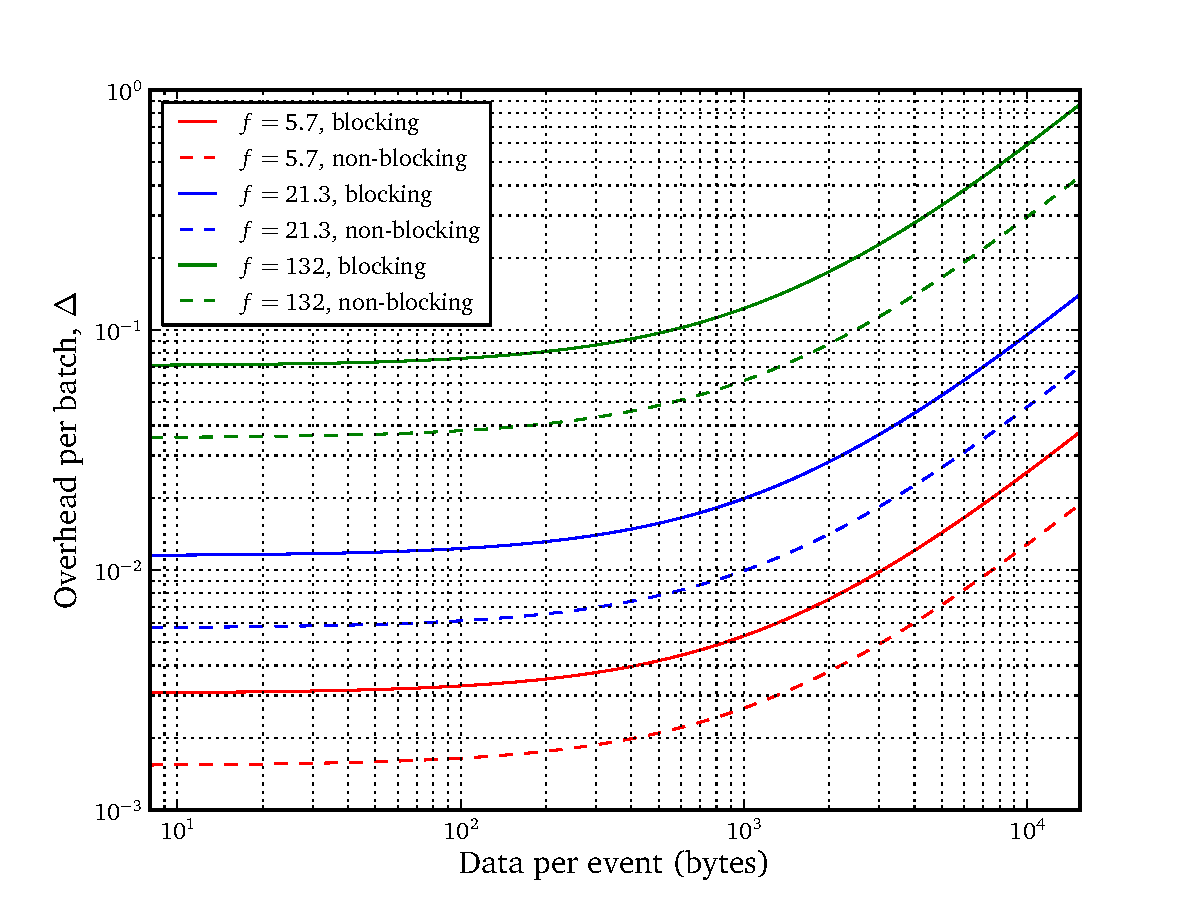
\includegraphics[width=4in]{figures/ch6/model_intrepid}
  \caption{Estimated tally server overhead for Intrepid Blue Gene/P
    supercomputer based on \eqref{eq:overhead-blocking} and
    \eqref{eq:overhead-nonblocking}.}
  \label{fig:model-intrepid}
\end{figure}

\begin{figure}[htb]
  \centering
  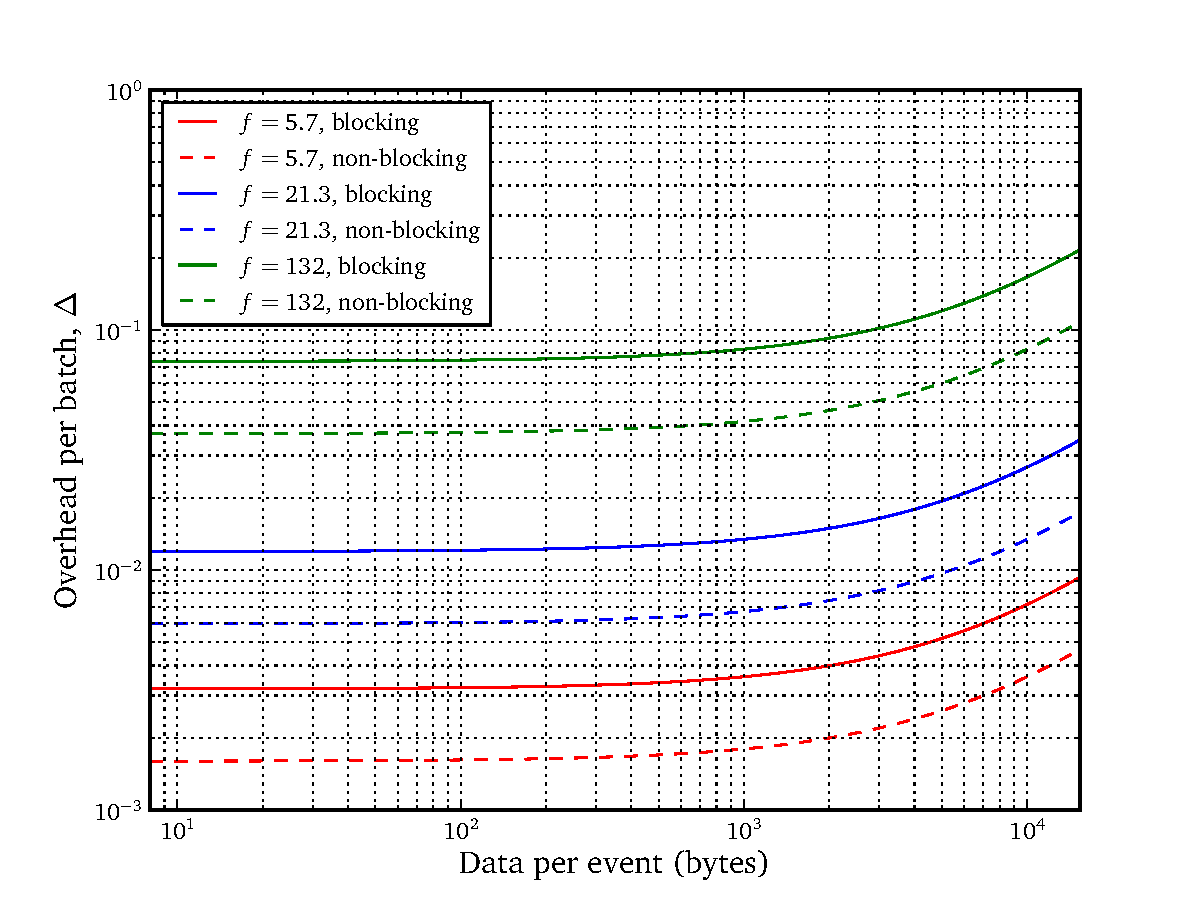
\includegraphics[width=4in]{figures/ch6/model_titan}
  \caption{Estimated tally server overhead for Titan Cray XK7 supercomputer
    based on \eqref{eq:overhead-blocking} and \eqref{eq:overhead-nonblocking}.}
  \label{fig:model-titan}
\end{figure}

We can also use equation \eqref{eq:support-ratio-blocking} to identify the
number of compute processors that can be supported by one server when using
blocking communication. For our worst case of $f = 21.3$ and $d = 15360$, the
constraint implies that on the Intrepid supercomputer we would need one server
for every 15 compute processors. On the Titan supercomputer, we would need one
server for every 58 compute processors for the same values of $f$ and $d$.

The predicted overhead due to tally servers based on the model in
\eqref{eq:overhead-blocking} and \eqref{eq:overhead-nonblocking} is quite
modest. In particular, over the range of parameter space that is of interest in
LWR analysis, the overhead is generally less than 10\% --- a very small price to
pay for the benefit of being able to have tallies of arbitrarily large size. The
promising results based on the theory presented here warrant an actual
implementation in a real Monte Carlo code. In \autoref{sec:implementation}, we
describe our implementation of this algorithm in the OpenMC Monte Carlo
code. Actual test results using the implementation in OpenMC are presented in
\autoref{sec:results}. Before we discuss the implementation and results,
however, we first discuss and analyze several considerations that may have an
influence on the achievable performance.

\subsection{Implications of total memory requirements}

One may have noted in the derivation of the performance model that, even though
the entire purpose of the algorithm is to allow for decomposition of the tally
memory, nowhere was the total memory requirement for the tallies taken into
account. In fact, one of the alluring aspects of the tally server algorithm is
that, in general, its performance does not depend on total amount of
memory. However, we must be careful in interpreting such a statement too broadly
as there are constraints on the memory.

The most obvious constraint is that the memory for each server must not exceed
the available memory on a single node. Let $M_t$ be the total memory required for
tallies, $M_s$ be the tally memory on each server, and $M_n$ be the available
memory on a node. This constraint implies that

\begin{equation}
  \label{eq:constraint-total}
  M_s < M_n.
\end{equation}

Another implicit assumption made in the course of the derivation was that the
message being sent was small relative to the tally memory on each
server. However, for a fixed tally size, the total tally memory on each server
will be inversely proportional to the total number of processors (assuming a
constant support ratio). Thus, as the total number of processors becomes very
large, the total memory on each server could hypothetically become smaller than
the message size for each scoring event. This situation would result in
increased overhead as it would necessitate sending more messages. A reasonable
constraint to impose is that the message size for each scoring event be smaller
that the tally memory of each server:

\begin{equation}
  \label{eq:constraint-message}
  d < M_s
\end{equation}

\noindent In practice, even $d = M_s$ can cause problems since a single message
can still overlap two servers. If we assume that the total memory required for
tallies is divided evenly over the tally servers, then the constraints in
\eqref{eq:constraint-total} and \eqref{eq:constraint-message} can be written in
combined form as

\begin{equation}
  \label{eq:constraint-memory}
  d < \frac{M_t}{s} < M_n.
\end{equation}

\noindent As we saw earlier, the upper limit on $d$ for our cases of interest is
15,360. Let us suppose that the memory on a single node is $M_n = 32 \cdot 10^9$
bytes. If the total memory of the tallies is $M_t = 500 \cdot 10^9$ bytes, then
\eqref{eq:constraint-memory} implies that

\begin{equation}
  \label{eq:constraint-example}
  15.6 < s < 3.26\cdot 10^6.
\end{equation}

\noindent Thus, we must have at least 16 servers in order for the memory
footprint of each to fit on a single node. This lower bound is quite easy to
achieve even on a small cluster. For the upper bound, if we have more the 3.26
million servers, each server would have too little data compared to the size of
a single message. At present, this limit puts no practical restrictions on our
use of the algorithm.

The constraint in \eqref{eq:constraint-memory} can also tell us, given a total
number of a tally servers, the range of total tally memory that can be
reasonably accommodated. Let us suppose we wanted to perform a simulation using
all nodes on the Mira Blue Gene/Q supercomputer at Argonne National
Laboratory. This supercomputer has 48 racks each having 1024 nodes, each of
which in turn has a 16 core processor for a total of 786,432 cores. Each node
has $M_n = 16 \cdot 10^9$ bytes of memory. Assuming a support ratio of $c/s =
15$, we would need 49,152 servers. Thus, \eqref{eq:constraint-memory} implies
that

\begin{equation}
  \label{eq:constraint-mira}
  755.0 \cdot 10^3 < M_t < 786.4 \cdot 10^{12}.
\end{equation}

\noindent For any reasonable simulation, the total memory of the tallies will
likely be somewhere between 755 kilobytes and 786 terabytes.

Admittedly, the foregoing analysis does not take into account the fact that
tally servers will have to share the memory of a single node with compute
processors. However, doing so would not change the overall conclusion that under
normal circumstances, the memory requirements are not a formidable challenge to
successfully employing the tally server algorithm.

\subsection{Dependence of \texorpdfstring{$\mu$ on $d$}{u on d}}

To this point, we have assumed that $\mu$ is independent of all other parameters
in our model. However, in most Monte Carlo transport codes, the rate at which
particles are simulated depends on how much data needs to be tallied. Hence
$\mu$ should really be a function of $d$, i.e. $\mu = \mu(d)$. In our case, $d$
will vary according to how many nuclides and scoring functions are being
tallied. For every nuclide reaction rate that needs to be tallied, it is
necessary to either calculate or look up a nuclide microscopic cross section at
the time of tallying. As a result, $\mu$ will depend linearly on $d$. If $\mu_0$
is the calculational rate with no tallies and $\mu_1$ is the average time to
process tally scores per byte, then we have that

\begin{equation}
  \label{eq:mu-function}
  \mu(d) = \mu_0 + d\mu_1
\end{equation}

\noindent Substituting $\mu(d)$ for $\mu$ in \eqref{eq:model-nonblocking}, the
tally server overhead using non-blocking communication would then be

\begin{equation}
  \label{eq:model-blocking-mud}
  \Delta_{\text{non-blocking}} = \frac{f}{\mu_0 + d\mu_1} \left ( \alpha + d\beta
    \right ).
\end{equation}

\noindent We see that the tendency would be to lessen the overhead as $d$ is
increased relative to the overhead in \eqref{eq:overhead-nonblocking}. In the
actual performance measurements discussed in \autoref{sec:results}, this effect
is accounted for explicitly by measuring $\mu$ over a range of $d$.

%%%%%%%%%%%%%%%%%%%%%%%%%%%%%%%%%%%%%%%%%%%%%%%%%%%%%%%%%%%%%%%%%%%%%%%%%%%%%%%%
\section{Implementation}
\label{sec:implementation}

\subsection{Description of algorithm}

The algorithm described in \autoref{sec:tally-server-algorithm} was implemented
in OpenMC; only modest changes were required to the source code to implement the
tally server algorithm. At initialization time, processes are divided into
compute processes and servers based on user input. If $p$ total processes and
$s$ servers are specified, then the processes whose MPI rank satisfies $i + 1
\mod s/p = 0$ are assigned as servers. Each user-defined tally has an array of
score objects whose length is the product of the number of filter bins
multiplied by the number of scoring functions. All scoring bins from
user-defined tallies are concatenated into one ``global'' tally score array
which is then divided equally over the servers. Finally, a look-up table is
constructed that relates indices in the global tally scores array to indices
within the scores array for each user-defined tally. The look-up table enables
the compute processes to determine which server they need to send scores to.

The necessary changes to the actual tallying subroutines that are used during
particle tracking follow directly from the discussion in
\autoref{sec:tally-server-algorithm}. As a summary, \autoref{alg:tallyserver}
shows a pseudocode outlining the salient points of the tally server algorithm as
implemented in OpenMC. There are a few important points to note regarding this
algorithm. Firstly, the array of scores created when a scoring event occurs
contains the scores for all specified scoring functions. This means that the
receiving server will increment multiple tally scores from a single
message. Also note that the servers must be informed of when a batch of
particles (or the simulation) has been completed as the servers are now
responsible for computing sums and sums of squares of the tally score bins in
order to calculate variances. At the end of the simulation, the servers must
collectively write the tally results to disk. This can be done efficiently using
parallel I/O techniques such as MPI-IO or parallel HDF5.

\begin{algorithm}
  \caption{Pseudocode for tally server algorithm}
  \label{alg:tallyserver}
  \begin{algorithmic}
    \If{compute process}
      \For{$i \gets 1 \textbf{ to } M$}
        \For{$j \gets 1 \textbf{ to } N/p$}
          \While{Particle $j$ is alive}
            \State Process next event
            \If{Event satisfies filter criteria}
              \State Create array for scores
              \ForAll{Scoring functions}
                \State Calculate score
                \State Add score to array
              \EndFor
              \State Determine server destination
              \State Send array to server
            \EndIf
          \EndWhile
        \EndFor
        \State Send `finished' message to server
      \EndFor
    \ElsIf{server}
      \Loop
        \State Receive message
        \If{End of batch}
          \State Accumulate tally scores
        \ElsIf{End of simulation}
          \State Accumulate tally scores
          \State {\bf exit loop}
        \Else
          \For{Score $i \gets 1 \textbf{ to } d$}
          \State Determine memory location $j$ to increment
          \State Increment tally $j$ with score $i$
          \EndFor
        \EndIf
      \EndLoop
      \State Write tally results to state point file
    \EndIf
  \end{algorithmic}
\end{algorithm}

\subsection{Potential optimizations}

\subsubsection{Explicit buffering}

In \autoref{alg:tallyserver}, an array of scores is sent to a server at every
single scoring event. If $f$ in \eqref{eq:overhead-blocking} or
\eqref{eq:overhead-nonblocking} is very large, this would clearly create a large
overhead regardless of whether the communication would be latency- or
bandwidth-dominated. One potential workaround for this situation would be to
explicitly buffer messages before sending. Rather than sending a message at
every scoring event, we could create a buffer array on the compute process for
each server that is some factor $\eta$ larger than the total number of scoring
functions for a tally. When the buffer array is full, it would then be sent to
the corresponding server. In this case, we have decreased $f$ by a factor of
$\eta$ and increased $d$ by the same factor. The predicted overhead using
non-blocking communication would then be
\begin{equation}
  \label{eq:overhead-nonblocking-buffer}
  \Delta_{\text{non-blocking}} = \frac{f}{\eta\mu} \left ( \alpha + d\eta\beta
  \right ) = \frac{f}{\mu} \left ( \frac{\alpha}{\eta} + d\beta \right ).
\end{equation}

\noindent We see in \eqref{eq:overhead-nonblocking-buffer} that the latency term
has been reduced by a factor of $\eta$, but the bandwidth term is
unchanged. Since the main case of interest (depletion of an LWR model) was shown
to be in the bandwidth-dominated region for contemporary supercomputers, the
extra effort of implementing explicit buffering did not seem to justify the
performance benefit for cases that are latency-dominated. This is especially
true given that, as we will see in \autoref{sec:results}, the overhead for
latency-dominated cases is extremely small. Explicit buffering could also
hypothetically limit network contention by reducing the total number of
messages, but this effect is hard to quantify.

\subsubsection{Combining successive scoring events}

A small variation on the explicit buffering concept described in the previous
section is to combine successive scores that match the same filter criteria. Let
us suppose that for a tally with scoring bins $b_i, i = 1, \dots, k$, we have
$n$ consecutive scoring events that match the same filter criteria. Let
$x_{i,j}$ be the $i$th score for the $j$th event. In the basic algorithm, we
send a message containing the values $x_{1,j}, x_{2,j}, \dots, x_{k,j}$ to a
server for each scoring event. Then the server adds each score to the
appropriate scoring bin $b_i \gets b_i + x_{i,j} \forall i$. Rather than sending
$n$ messages and having the server accumulate each array of scores, the compute
processes can combine consecutive scores and subsequently send the sum to a
server to be accumulated. Each compute process would calculate $x_i' = \sum_j
x_{i,j}$, and the server would accumulate $b_i \gets b_i + x_i'$. This scheme
effectively reduces the number of scoring events per particle, $f$.

To obtain a simple estimate of the potential reduction in $f$, let us consider
the case of track-length tallies in the fuel region. Any time a particle
scatters within the fuel region, it will result in two separate tracks. The
tally scores from these separate tracks could be combined and sent to a server
in one message. This implies that the effective number of scoring events, $f'$,
is then
\begin{equation}
  f' = \left ( 1 - \frac{\Sigma_s \phi}{\Sigma_t \phi} \right ) f
\end{equation}
where $\Sigma_s \phi$ is the scattering reaction rate in the fuel and $\Sigma_t
\phi$ is the total reaction rate in the fuel. For the Monte Carlo performance
benchmark $\Sigma_s \phi/\Sigma_t \phi = 0.23$, so $f$ would be reduced about
23\%.

\subsubsection{Topologically-aware layouts}

To maximize network bandwidth and minimize latency, the mapping of processes to
processor cores could hypothetically be optimized based on the topology of the
particular machine the algorithm is implemented on. We chose a naïve
implementation that is unaware of topology to ensure portability across
different architectures and to demonstrate that successful use of the algorithm
does not require such optimizations.

%%%%%%%%%%%%%%%%%%%%%%%%%%%%%%%%%%%%%%%%%%%%%%%%%%%%%%%%%%%%%%%%%%%%%%%%%%%%%%%%
\section{Results}
\label{sec:results}

The performance model developed in \autoref{sec:tally-server-analysis} is dependent on a
variety of parameters. On any given computer, $\alpha$, $\beta$, and $\mu$ are
effectively constant. The remaining parameters can be manipulated by varying the
definition of the tallies and the job parameters. Thus, to fully test the
performance of the tally server implementation, a parameter study should be
carried out by running a series of simulations varying the parameters $p$, $s$,
$f$, and $d$.

One could argue that based on \eqref{eq:overhead-nonblocking}, it should not be
necessary to include $p$, $c$, or $s$ in the parameter study since the overhead
does not explicitly depend on those parameters. However,
\eqref{eq:overhead-nonblocking} was derived assuming that the support ratio
attains its maximum based on the inequality in
\eqref{eq:support-ratio-nonblocking}. In practice, it's not possible to know
\emph{a priori} what the maximum attainable support ratio is and thus it is
instructive to test this directly. While the performance depends on $f$ in
general, our primary interest is tally events in the fuel region. As a result,
we performed a parameter study using the modified version of OpenMC varying $p$,
$c/s$, and $d$ only.

First, a number of ``baseline'' simulations of the Monte Carlo performance
benchmark were run to determine how $\mu$ varies with increasing $d$, and hence
how $t_0$ varies with increasing $d$. The baseline simulations were run without
tally servers to capture only the increase in simulation time due to cross
section look-ups for tallies. On both the Titan supercomputer, the baseline
simulations were run with 16 processors with a total of 32,000 particles per
batch. Ten batches were run both without tallies (referred to as \emph{inactive
  batches}) and with tallies (\emph{active batches}). These values were found to
be adequate to accurately profile performance. On the Intrepid supercomputer,
the baseline simulation was run with a single processor with 2000 particles per
batch. Again, ten batches were run first without and then with tallies. For each
case, a tally was set up with a mesh filter and a second filter to match only
events within the fuel volume. The scoring functions requested were the flux,
total reaction rate, scattering rate, absorption rate, fission rate, and neutron
production rate for varying numbers of nuclides, starting with 5 nuclides and
doubling the number of nuclides up to 320. Thus, the amount of data sent at each
event varied from 240 bytes up to 15.36 kilobytes. \autoref{fig:mu-d} shows the
observed dependence of $\mu$ on $d$ normalized to the $d=5$ case.

\begin{figure}
  \centering
  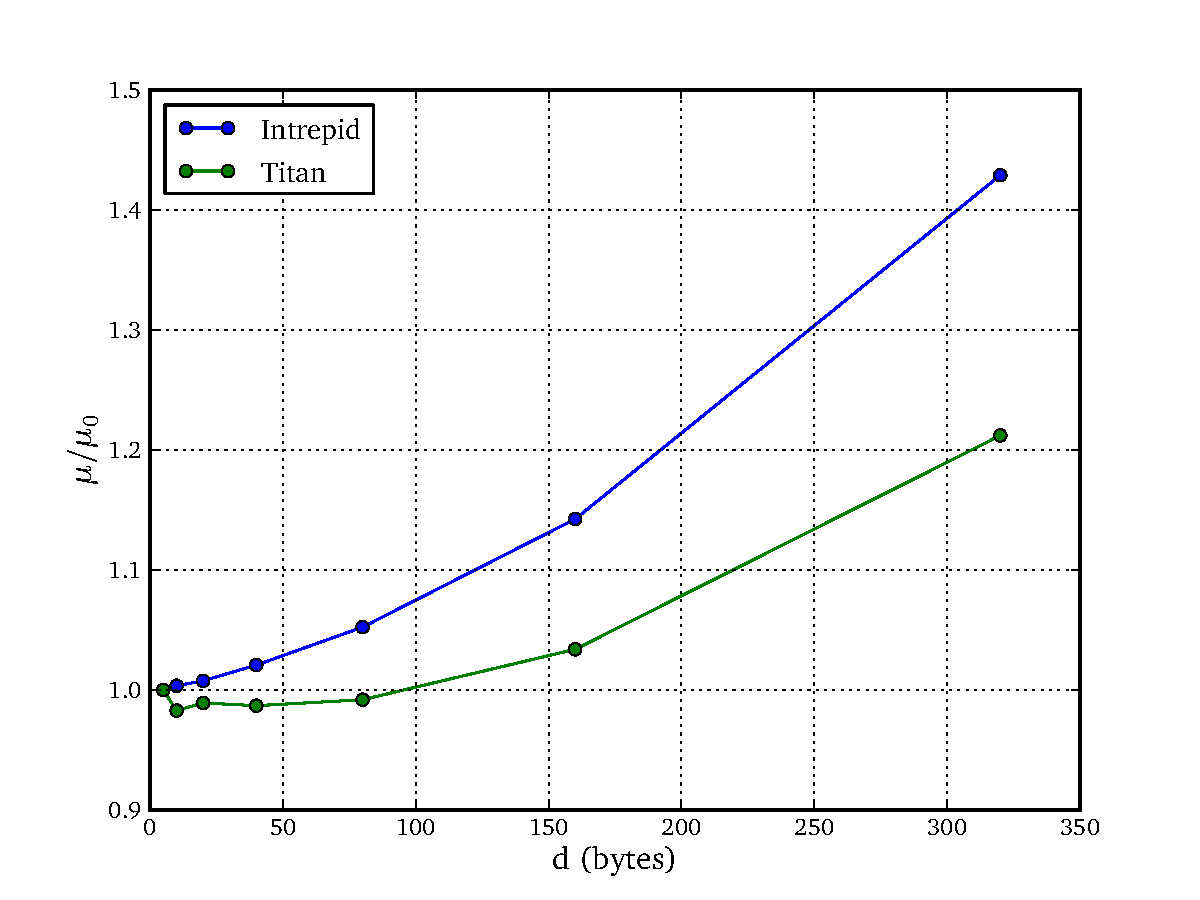
\includegraphics[width=4.0in]{figures/ch6/results_baseline.pdf}
  \caption{Observed dependence of $\mu$ on the amount of data tallied, $d$, on
    Intrepid and Titan.}
  \label{fig:mu-d}
\end{figure}

The parameter study using tally servers on the Intrepid supercomputer consisted
of 168 simulations with each combination of the following parameters: $p =
16,32,64,128, \allowbreak 256,512$, $c/s = 1,3,7,15$, and $d = 240, 480, 960,
1920, 3840, 7680, 15360$. Like the baseline cases, the runs with tally servers
had 10 inactive batches, 10 active batches, and $N/p = 500$. The effective
overhead from tally servers was determined in the following manner. First, the
expected overhead due to looking up cross sections during tallying was
subtracted from the active batch time based on the results from the baseline
cases. Then, the adjusted simulation time in active batches was divided by the
inactive batch time to determine the overhead in active batches. This
essentially represents an estimate for the second term in \eqref{eq:model},
i.e. it does not account for the fact that we have fewer compute
processors. However, if we know $p$ and $c$, that source of overhead is trivial
to calculate --- it is really the extra overhead from message-passing that we
are interested in. The overhead calculated in this manner for $c/s = 1$, $c/s =
3$, $c/s = 7$, and $c/s = 15$ is shown in \autoref{fig:intrepid-r1},
\autoref{fig:intrepid-r3}, \autoref{fig:intrepid-r7}, and
\autoref{fig:intrepid-r15}, respectively.

\begin{figure*}[!th]
  \makebox[\textwidth][c]{
  \begin{floatrow}[2]
    \ffigbox[\FBwidth] {
          \caption{Tally server overhead on Intrepid Blue Gene/P as a function
            of data per event with $c/s = 1$.}
          \label{fig:intrepid-r1}
        } {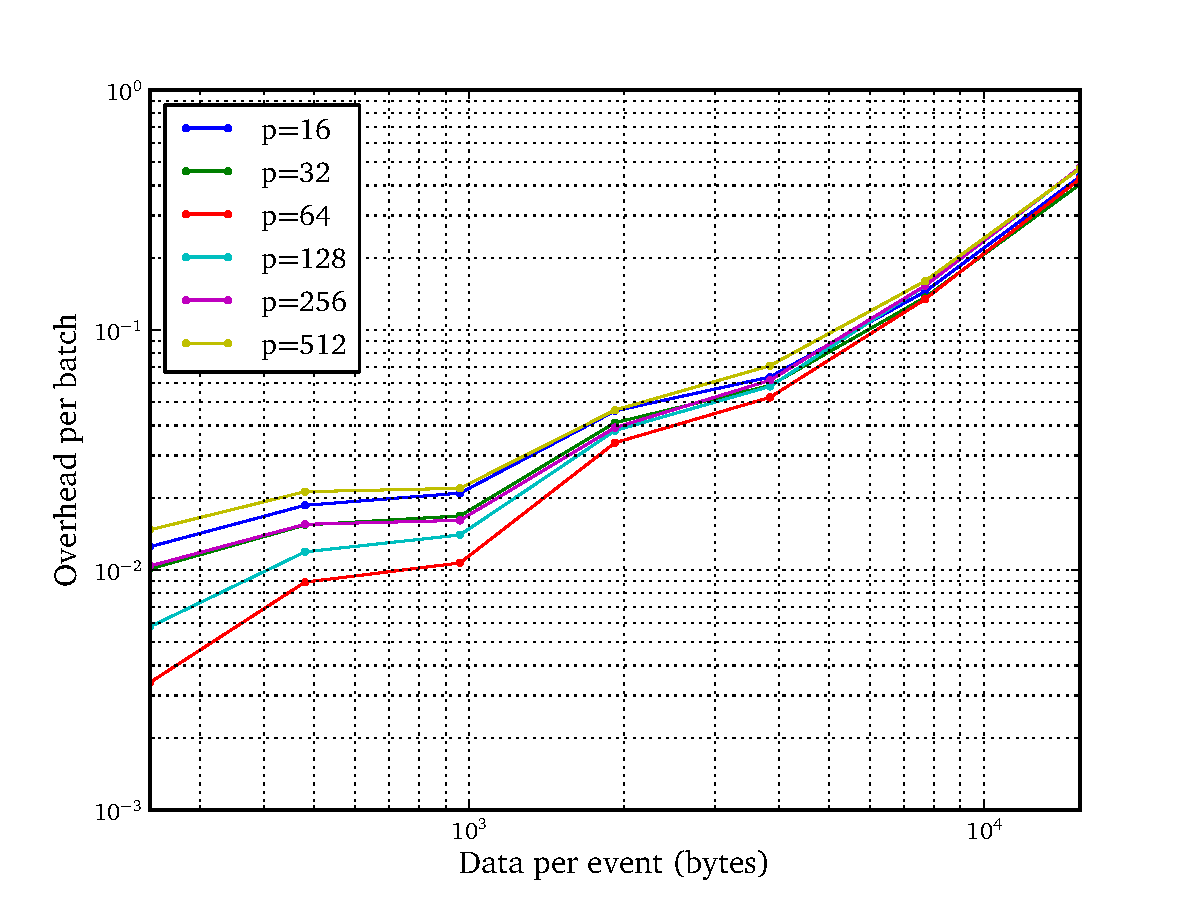
\includegraphics[width=3.4in]{figures/ch6/results_intrepid_r1}}
    \ffigbox[\FBwidth] {
          \caption{Tally server overhead on Intrepid Blue Gene/P as a function
            of data per event with $c/s = 3$.}
          \label{fig:intrepid-r3}
        } {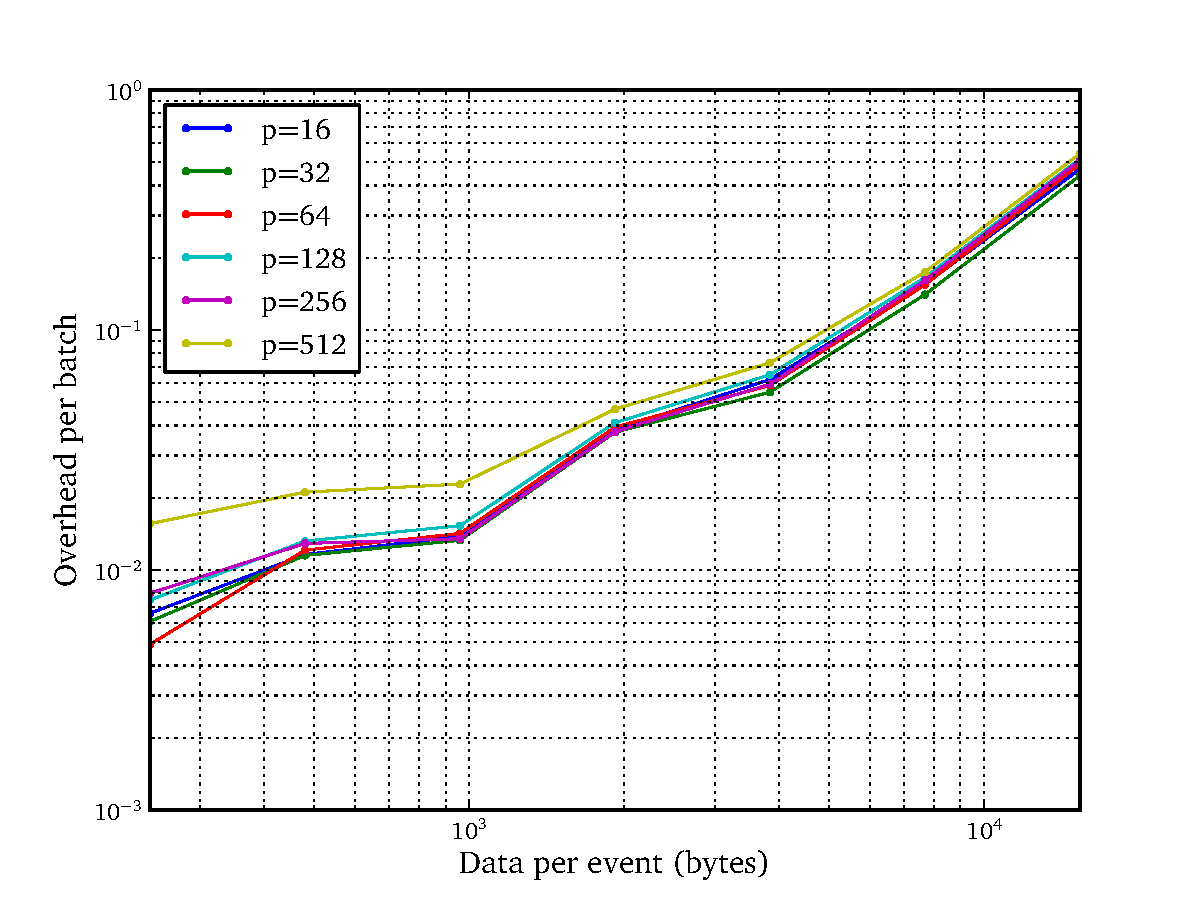
\includegraphics[width=3.4in]{figures/ch6/results_intrepid_r3}}
  \end{floatrow}
  }
  \begin{floatrow}
    \ffigbox[\FBwidth] {
          \caption{Tally server overhead on Intrepid Blue Gene/P as a function
            of data per event with $c/s = 7$.}
          \label{fig:intrepid-r7}
        } {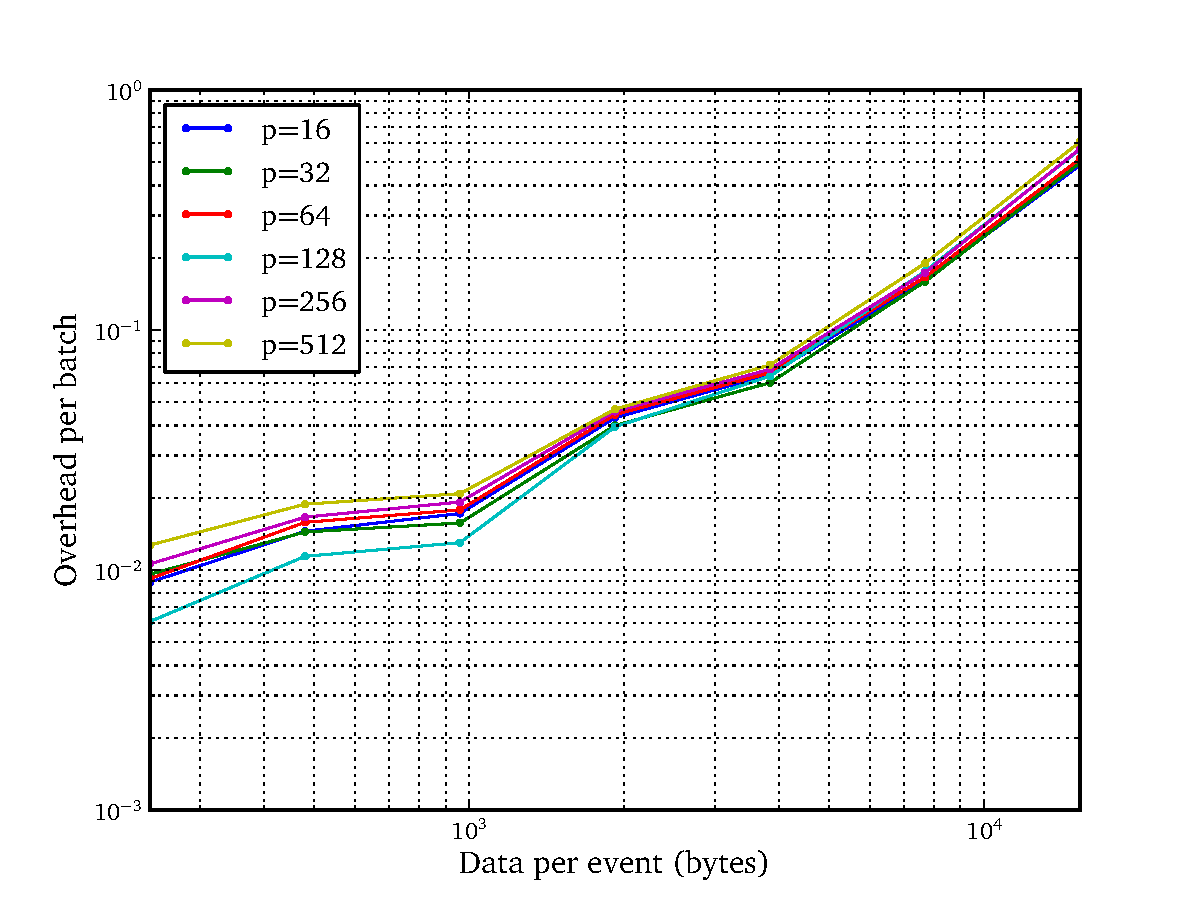
\includegraphics[width=3.4in]{figures/ch6/results_intrepid_r7}}
    \ffigbox[\FBwidth] {
          \caption{Tally server overhead on Intrepid Blue Gene/P as a function
            of data per event with $c/s = 15$.}
          \label{fig:intrepid-r15}
        } {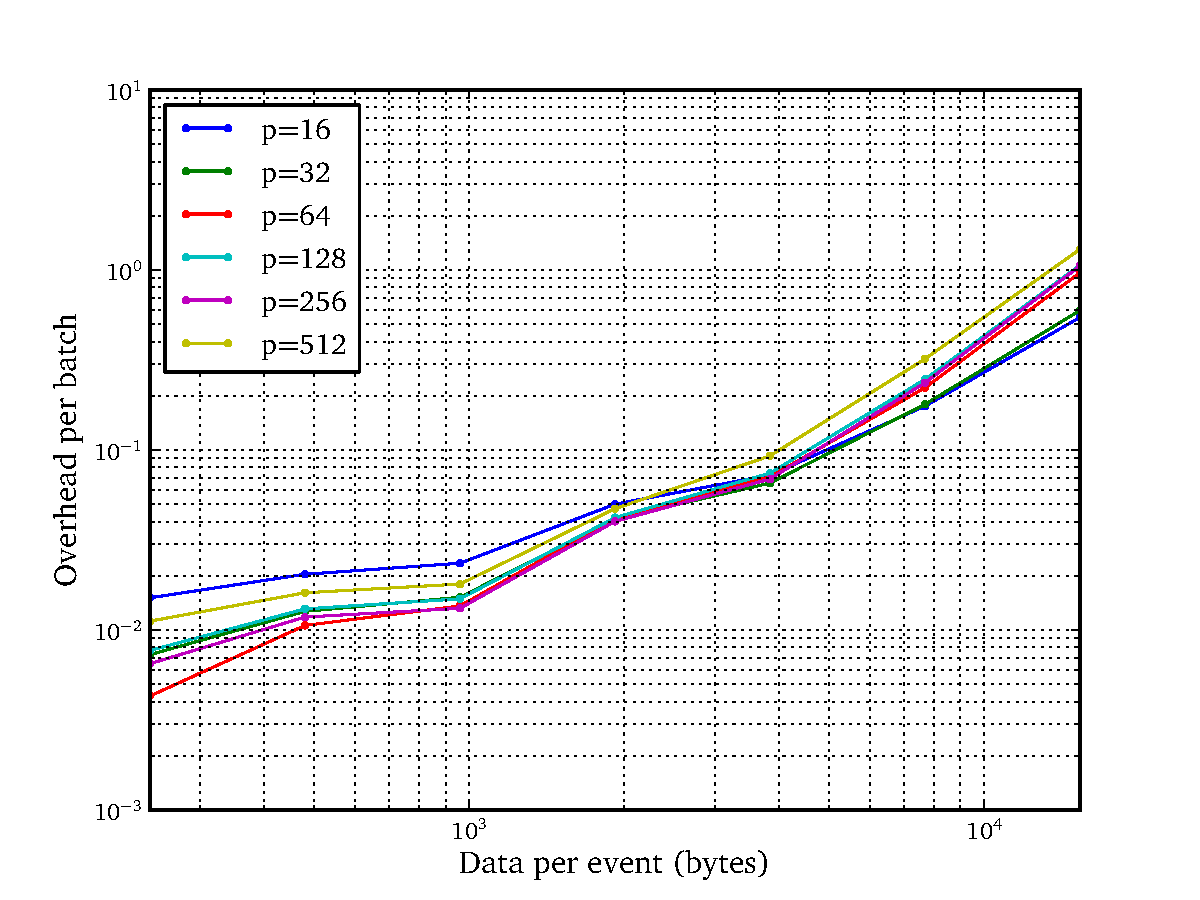
\includegraphics[width=3.4in]{figures/ch6/results_intrepid_r15}}
  \end{floatrow}
\end{figure*}

It is also of interest to observe the behavior of the tally server overhead with
increasing numbers of total processors. Recall that the performance model
predicts that the overhead should not depend on the number of processors
used. \autoref{fig:intrepid-cs} shows the overhead plotted as a function of $p$
for cases with $d = 15360$. We see that the overhead does not increase
appreciably for $c/s = 1, 3, 7$. However, for $c/s = 15$ the performance begins
to degrade. This may indicate that on Intrepid, this support ratio is not quite
sufficient for all servers to keep up with the volume of messages. Since the
model assumptions regarding achievable bandwidth do not account for contention,
such deviation from the model is not unexpected.

\begin{figure}[!tbh]
  \centering
  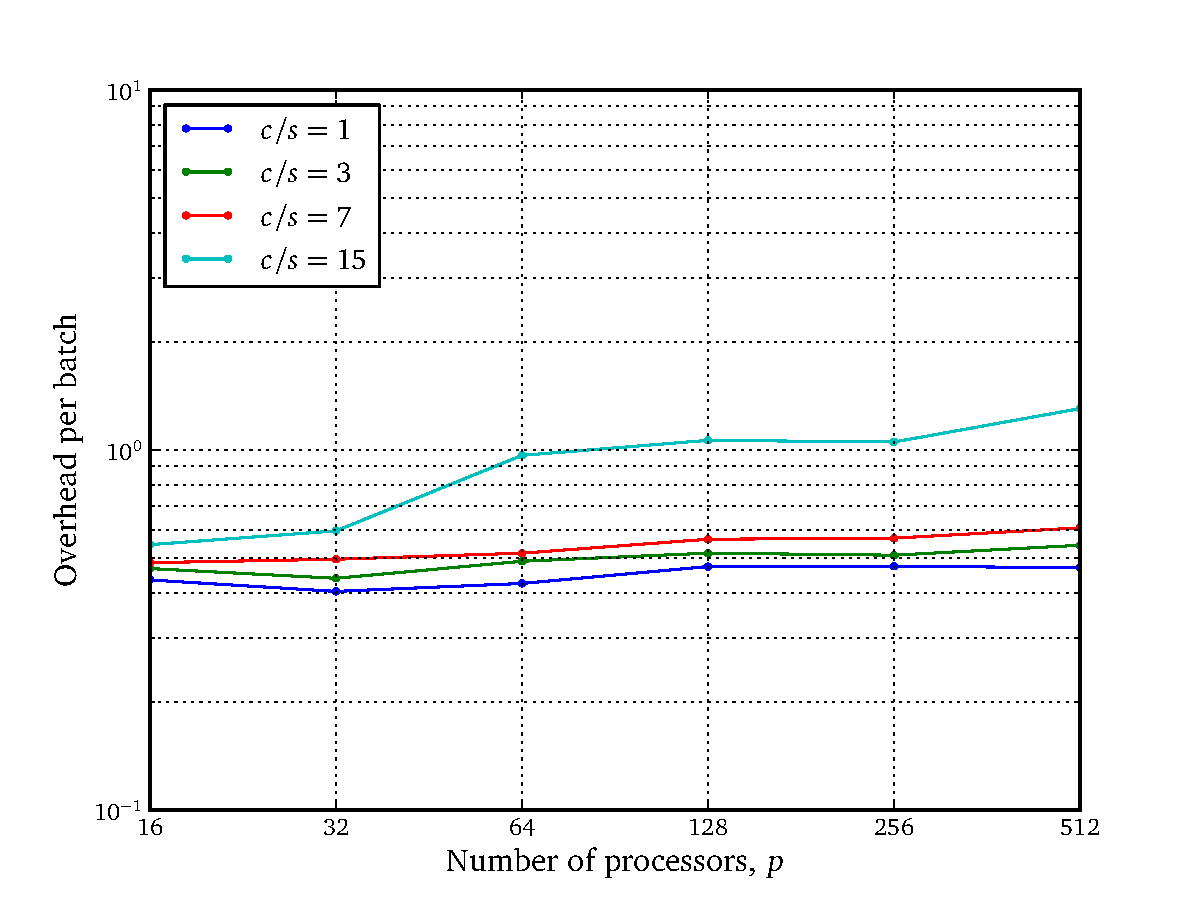
\includegraphics[width=4in]{figures/ch6/results_intrepid_cs}
  \caption{Tally server overhead on Intrepid Blue Gene/P as a function of $p$
    for $d = 15360$.}
  \label{fig:intrepid-cs}
\end{figure}

Another parameter study using tally servers on the Titan supercomputer consisted
of 196 simulations with each combination of the following parameters: $p =
16,32,64,128,256,512,1024$, $c/s = 1,3,7,15$, and $d = 240, 480, 960, 1920,
3840, 7680, \allowbreak 15360$. Again, the runs with tally servers had 10
inactive batches, 10 active batches, and $N/p = 1000$. The effective overhead
from tally servers was determined as described for the study on Intrepid. The
calculated overhead for $c/s = 1$, $c/s = 3$, $c/s = 7$, and $c/s = 15$ is shown
in \autoref{fig:titan-r1}, \autoref{fig:titan-r3}, \autoref{fig:titan-r7}, and
\autoref{fig:titan-r15}, respectively.

\begin{figure*}[!tbh]
  \makebox[\textwidth][c]{
  \begin{floatrow}[2]
    \ffigbox[\FBwidth] {
          \caption{Tally server overhead on Titan Cray XK7 as a function
            of data per event with $c/s = 1$.}
          \label{fig:titan-r1}
        } {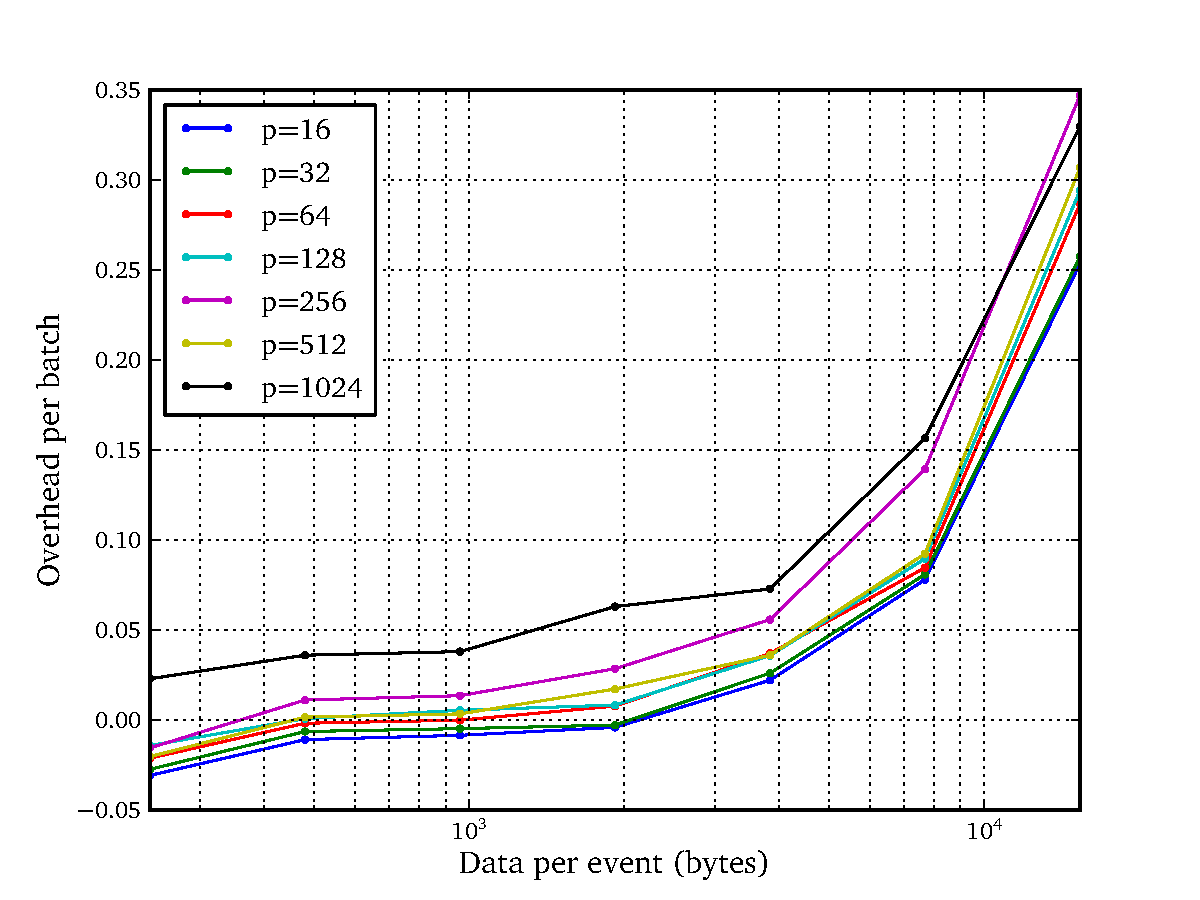
\includegraphics[width=3.4in]{figures/ch6/results_titan_r1}}
    \ffigbox[\FBwidth] {
          \caption{Tally server overhead on Titan Cray XK7 as a function
            of data per event with $c/s = 3$.}
          \label{fig:titan-r3}
        } {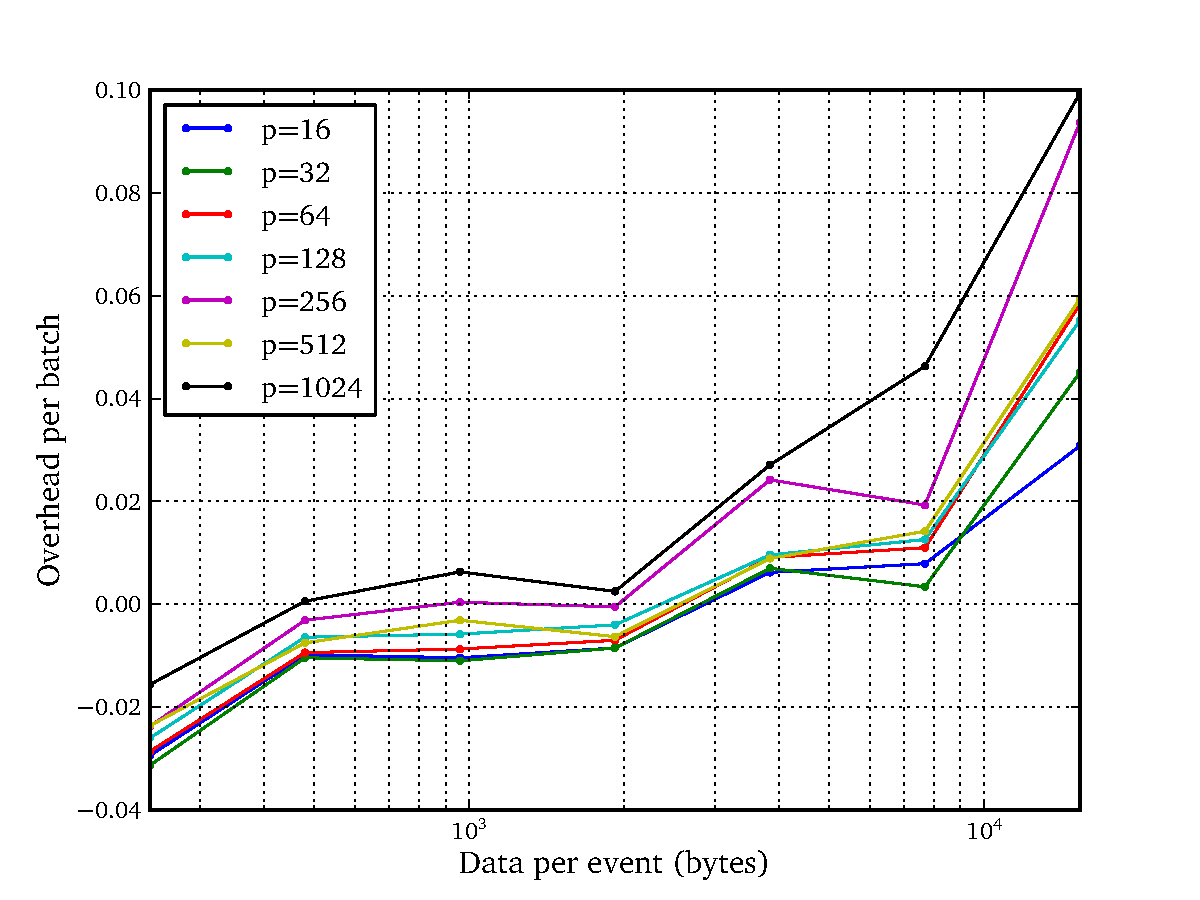
\includegraphics[width=3.4in]{figures/ch6/results_titan_r3}}
  \end{floatrow}
  }
  \begin{floatrow}
    \ffigbox[\FBwidth] {
          \caption{Tally server overhead on Titan Cray XK7 as a function
            of data per event with $c/s = 7$.}
          \label{fig:titan-r7}
        } {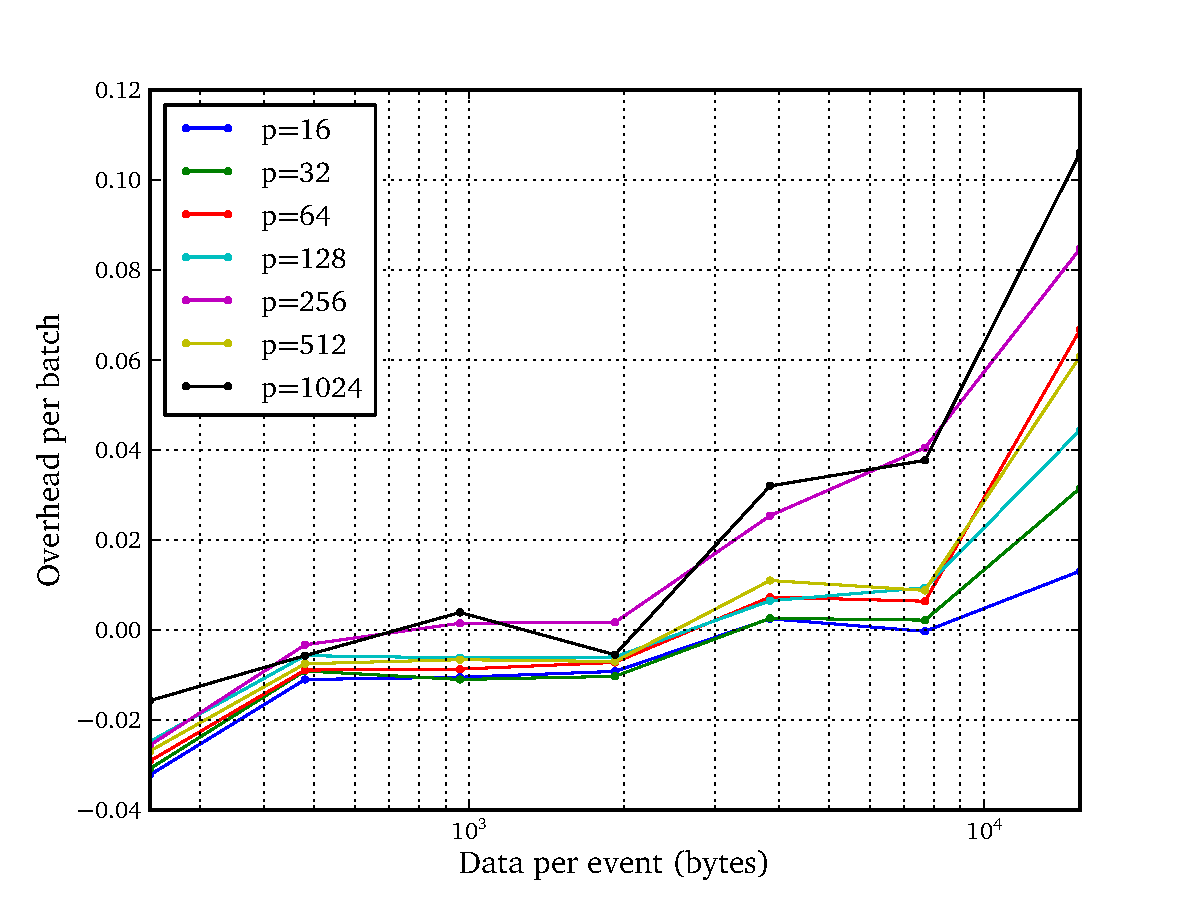
\includegraphics[width=3.4in]{figures/ch6/results_titan_r7}}
    \ffigbox[\FBwidth] {
          \caption{Tally server overhead on Titan Cray XK7 as a function
            of data per event with $c/s = 15$.}
          \label{fig:titan-r15}
        } {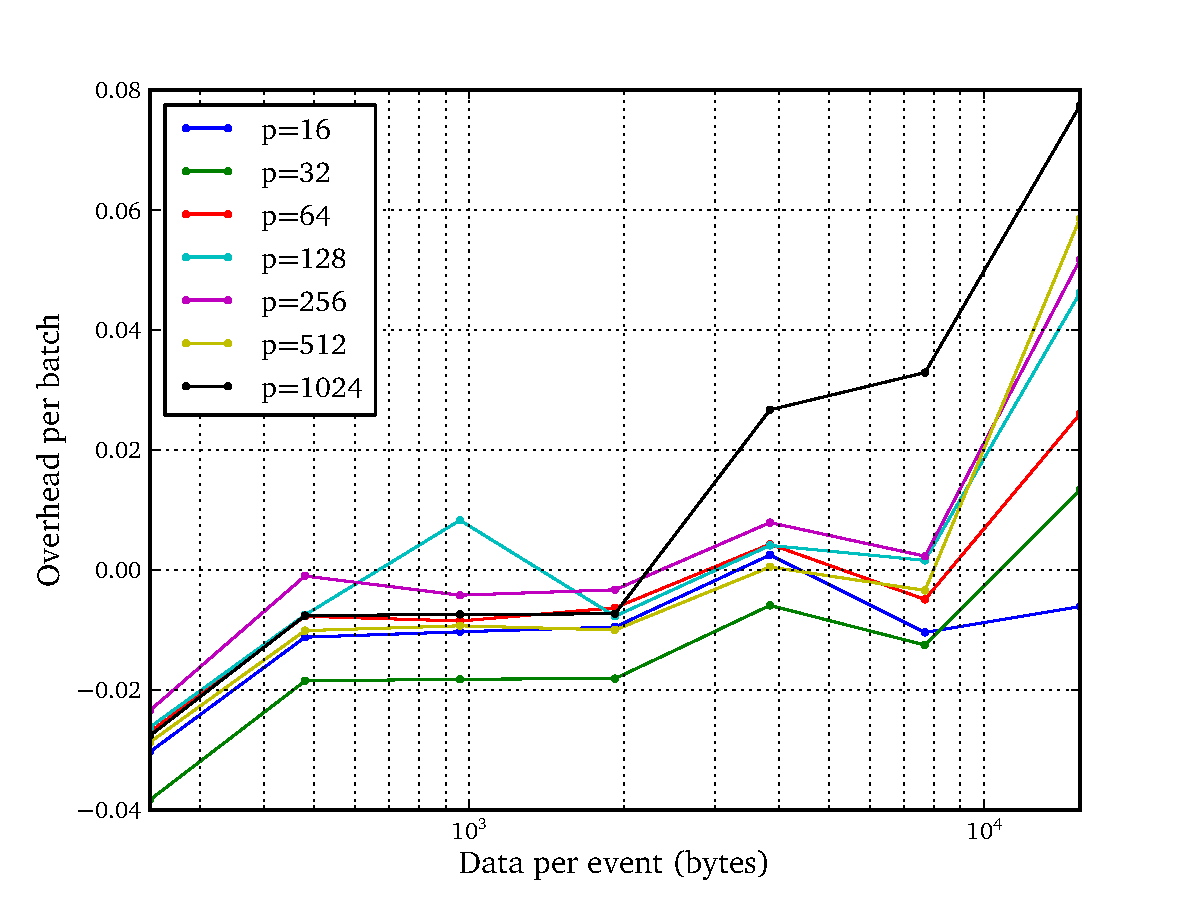
\includegraphics[width=3.4in]{figures/ch6/results_titan_r15}}
  \end{floatrow}
\end{figure*}

Similar to \autoref{fig:intrepid-cs}, we can look at the behavior of the tally
server overhead on Titan with increasing $p$. \autoref{fig:titan-cs} shows the
overhead plotted as a function of $p$ for cases with $d = 15360$. We see that
the overhead is relatively stable with increasing $p$. However, the cases with
$c/s = 1$ are clearly outliers with much higher overhead than the other
cases. This is likely due to network contention since the $c/s = 1$ cases result
in half of the processor cores on each node sending messages simultaneously. To
understand in greater depth the variability of the overhead as a function of,
e.g., the support ratio would likely require a deeper investigation of a
particular architecture, including topology-aware algorithms and a more
sophisticated model for network contention. These studies are beyond the scope
of the present work and are not central to addressing the key questions we set
out to study.

\begin{figure}[!tbh]
  \centering
  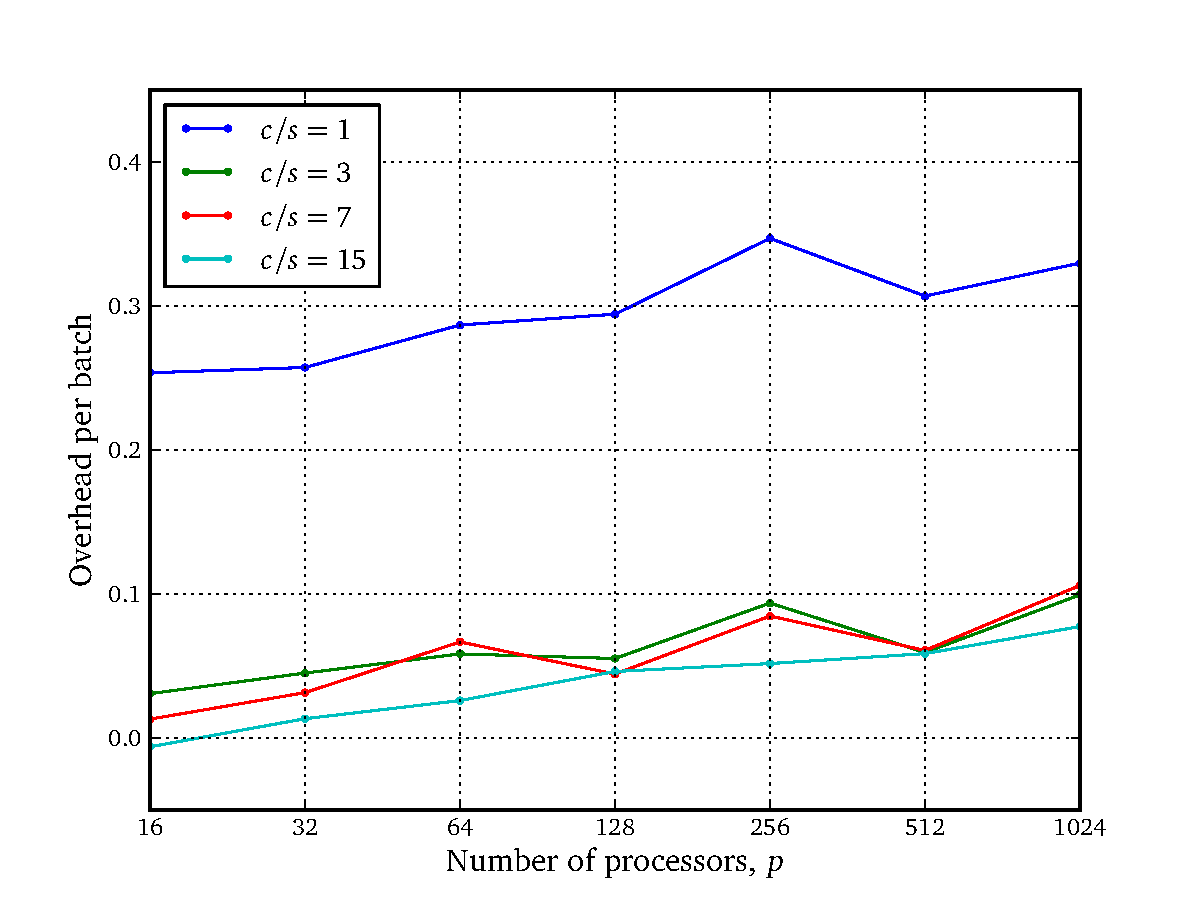
\includegraphics[width=4in]{figures/ch6/results_titan_cs}
  \caption{Tally server overhead on Titan Cray XK7 as a function of $p$ for $d =
    15360$.}
  \label{fig:titan-cs}
\end{figure}

%%%%%%%%%%%%%%%%%%%%%%%%%%%%%%%%%%%%%%%%%%%%%%%%%%%%%%%%%%%%%%%%%%%%%%%%%%%%%%%%
\section{Conclusions}

An algorithm for decomposing large tally data in Monte Carlo particle transport
simulations was proposed, analyzed, and implemented/tested in OpenMC. The
algorithm relies on disjoint sets of compute processes and servers of which the
former simulate particles moving through the geometry and the latter runs in a
continuous loop receiving scores from the compute processors and incrementing
tallies. This algorithm potentially allows the end user to dramatically increase
the overall tally memory footprint and therefore enables the potential to carry
out full core fuel depletion calculations.

The proposed algorithm is only of practical value if the communication penalty
resulting from tally decomposition is reasonable relative to the key timescales
of the problem. We carried out an analysis to that end and showed in
\autoref{sec:tally-server-analysis} that for a range of parameters relevant to 
LWR analysis, the tally server algorithm should perform with minimal overhead on
contemporary supercomputers regardless of the message-passing semantics. An
implementation of the algorithm in OpenMC was tested on the Intrepid and Titan
supercomputers and was demonstrated to perform well over a wide range of the
parameters. We can conclude that even with no further improvements in the
algorithm or its implementation in OpenMC, it could be successfully used to
analyze LWR models with a level of fidelity that was heretofore not possible due
to the need to replicate memory across all processors. It is likely that future
developments in Monte Carlo methods for reactor analysis and improvements in
computer architectures will only improve the performance of the tally server
algorithm over time.

One point that was made earlier was that the algorithm presented here does not
reduce the burden of large cross section data. For realistic reactor analysis,
cross section data may well reach into the hundreds of gigabytes owing to the
fact that cross section libraries would be needed at a multitude of
temperatures. In \autoref{sec:cross-section-memory}, we had discussed two
promising efforts in the area of on-the-fly evaluation of effective cross
sections at any temperature --- the work of Yesilyurt on on-the-fly Doppler
broadening \cite{nse-yesilyurt-2012} and the work of Viitanen on explicit
temperature treatment \cite{nse-viitanen-2012}. The latter development would
enable simulation using 0 K cross sections but with a significant performance
penalty. In general, this and other improvements in physics methods will likely
lead to slower simulations but with higher fidelity. From the perspective of the
tally server model, these developments will increase $\mu$ and consequently
decrease the communication overhead.

On the hardware end, improvements in supercomputer architectures may continue to
reduce network latency and improve bandwidth, at least in the short-term. Again,
this will largely benefit the tally server algorithm. Since incrementing tallies
can naturally be expressed as a fetch-and-add atomic operation, there is also
potential to exploit remote direct memory access (RDMA) operations either
explicitly (e.g., using MPI-2) or implicitly through a partitioned global
address space (e.g., Fortran co-arrays). Modern network interconnects should be
able to take advantage of RDMA operations. In addition, the requirement that
servers and compute processes be disjoint could be obviated by the use of RDMA,
potentially offering further reductions in overhead.

One potential downside to the algorithm presented here is that it considerably
complicates the use of threading via OpenMP. The most natural means of obtaining
thread-level parallelism in a Monte Carlo particle transport simulation is to
divide particles within a batch over multiple threads. Normally, no
communication occurs until the end of a batch when it is necessary to
synchronize fission bank sites and tallies. However, with the inclusion of tally
servers, it would then be necessary for each thread to participate in
message-passing. Further algorithmic innovations will need to be explored to
efficiently combine a tally server model with on-node shared-memory parallelism.

As a final comment, one should recognize the fact that the algorithm presented
here has primarily been presented with a focus and intent on applications in LWR
analysis. For other types of analysis performed with Monte Carlo, it may turn
out that the tally server algorithm does not make sense.
